\documentclass{article}
\usepackage{graphicx}
\graphicspath{ {images_latex/} }

\title{Assignment 1 Geo1001}
\author{Lisa Geers}

\begin{document}

\maketitle

\section{A1}

    \subsection{Mean statistics}

        In table 1 the calculated mean statistics of all sensors are displayed. The means of the sensors are
        quite similar for all variables. The means of the wind variables Direction - True, Wind Speed, 
        Crosswind Speed and Headwind Speed differ the most between sensors. This is logical, because 
        wind can differ greatly over short distances. This is in contrast with other variables 
        like Temperature and Relative Humidity, which are less dynamic and thus have a similar mean for all 
        sensors


        \begin{table}[h]
            \caption {Mean Statistics of all sensors}
            \resizebox{\columnwidth}{!}{%
            \begin{tabular}{llllllllllllllll}
            \hline
                                        & Mean A              & Mean B               & Mean C              & Mean D              & Mean E              & Standard Devation A & Standard Devation B & Standard Devation C & Standard Devation D & Standard Devation E & Variance A         & Variance B         & Variance C         & Variance D         & Variance E          \\ \hline
            Direction - True             & 209.40630048465266  & 183.41235864297255   & 183.58892481810832  & 198.32659660468877  & 223.95636363636365  & 100.54322606601899  & 99.88602389941525   & 87.76880480018731   & 90.18808156618324   & 96.47945418449655   & 10108.940307762601 & 9977.217770434554  & 7703.363096053383  & 8133.890056588521  & 9308.285079738369   \\
            Wind Speed                   & 1.290306946688207   & 1.242124394184168    & 1.3714632174616006  & 1.5816491511721908  & 0.5962424242424242  & 1.118550173932421   & 1.1408337241403745  & 1.1962107079801148  & 1.31902114073203    & 0.7150012449874839  & 1.2511544916042492 & 1.3015015861359962 & 1.4309200578862873 & 1.7398167696980256 & 0.5112267803336519  \\
            Crosswind Speed              & 0.9649434571890144  & 0.8356219709208401   & 0.9632983023443816  & 1.2105092966855295  & 0.4385050505050505  & 0.9625968857618368  & 0.9373287085891301  & 1.0210655229734091  & 1.2047833560489647  & 0.562087167714658   & 0.9265927644783866 & 0.8785851079453664 & 1.0425748022049617 & 1.4515029350126065 & 0.3159419841094861  \\
            Headwind Speed               & 0.16352988691437803 & -0.12980613893376414 & -0.2628940986257074 & -0.3005658852061439 & 0.19494949494949496 & 1.017320058054766   & 1.1210349307394734  & 1.127711035165007   & 1.1101813871607582  & 0.5648655661268653  & 1.0349401005205527 & 1.2567193159380559 & 1.2717321788329317 & 1.232502712398185  & 0.31907310779582404 \\
            Temperature                  & 17.96910339256866   & 18.065428109854604   & 17.91313662085691   & 17.99636216653193   & 18.353939393939395  & 3.9829975215127065  & 4.077875295758688   & 4.013046004830651   & 4.013177206370107   & 4.363843742775605   & 15.864269256376364 & 16.629066927759013 & 16.104538236887244 & 16.105591289728583 & 19.0431322113618    \\
            Globe Temperature            & 21.544588045234246  & 21.799434571890146   & 21.587388843977365  & 21.359296685529507  & 21.176161616161615  & 8.257805550937451   & 8.127073080259526   & 8.242651557816295   & 7.823186869859439   & 7.950817734146231   & 68.19135251709339  & 66.04931685187906  & 67.9413047035714   & 61.20225280074113  & 63.21550264161421   \\
            Wind Chill                   & 17.838206785137317  & 17.945920840064623   & 17.77299919159256   & 17.835367825383994  & 18.2940202020202    & 4.032920371452324   & 4.127447852847276   & 4.06707790227351    & 4.069011197957792   & 4.374592786175935   & 16.264446722475153 & 17.035825777973596 & 16.541122663161495 & 16.556852129105906 & 19.137062044862528  \\
            Relative Humidity            & 78.18477382875606   & 77.87831179321486    & 77.96285367825384   & 77.94203718674213   & 76.7930505050505    & 19.390978804050324  & 20.214425745479723  & 19.355170964011418  & 19.74477248514976   & 20.16170782941016   & 376.0100589791289  & 408.62300821951345 & 374.6226430461106  & 389.8560404903271  & 406.49446259849907  \\
            Heat Stress Index            & 17.899596122778675  & 18.00428109854604    & 17.82825383993533   & 17.92162489894907   & 18.286424242424246  & 3.8725764449092246  & 3.929269324233937   & 3.9187055976553324  & 3.88814143003908    & 4.2982833827256695  & 14.99684832166577  & 15.439157422365822 & 15.356253561095237 & 15.117643779986343 & 18.475240038215624  \\
            Dew Point                    & 13.553877221324719  & 13.530856219709205   & 13.458124494745352  & 13.50860953920776   & 13.558787878787879  & 3.118248198871891   & 3.1042741850691207  & 3.17555498985501    & 3.1736230057997945  & 3.069623011701569   & 9.723471829767792  & 9.636518216086554  & 10.084149493593053 & 10.071882982941721 & 9.42258543396781    \\
            Psychro Wet Bulb Temperature & 15.270718901453955  & 15.295516962843294   & 15.196645109135003  & 15.26018593371059   & 15.406666666666666  & 2.63515220041187    & 2.6019728519991188  & 2.690597228681732   & 2.6541294009257097  & 2.645268499131606   & 6.944027119335519  & 6.770262722540429  & 7.239313446989817  & 7.044402876858267  & 6.997445432497979   \\
            Station Pressure             & 1016.1682552504037  & 1016.6570274636512   & 1016.689329021827   & 1016.7280113177042  & 1016.1661010101009  & 6.202520988371144   & 6.069755714457117   & 6.139339656821912   & 5.915047217819551   & 6.240185369824895   & 38.47126661118455  & 36.841934433184825 & 37.69149142182619  & 34.98778358903481  & 38.93991344977666   \\
            Barometric Pressure          & 1016.1284329563813  & 1016.6164781906298   & 1016.6518997574777  & 1016.6888843977364  & 1016.127797979798   & 6.202253690096152   & 6.068679242921268   & 6.1380471779360235  & 5.912049294318023   & 6.239805833414894   & 38.467950836311324 & 36.82886775346346  & 37.67562315856838  & 34.952326858446234 & 38.93517683871854   \\
            Altitude                     & -25.98707592891761  & -30.05815831987076   & -30.338722716248988 & -30.653193209377527 & -25.96121212121212  & 51.6104741793961    & 50.45501096417206   & 51.07381554372864   & 49.19068601563611   & 51.88789247750703   & 2663.6410450221115 & 2545.708131394723  & 2608.5346341948175 & 2419.723590688898  & 2692.3533857573307  \\
            Density Altitude             & 137.31663974151857  & 135.58077544426493   & 129.62287793047696  & 132.41107518189168  & 150.84              & 162.8190539993073   & 163.90030579705498  & 164.2759963297163   & 162.83772822207789  & 172.380183031638    & 26510.04434522935  & 26863.310240368137 & 26986.602970120963 & 26516.1257325273   & 29714.92750202102   \\
            NA Wet Bulb Temperature      & 15.981542810985461  & 15.996809369951535   & 15.934236054971707  & 15.915642683912694  & 15.93688888888889   & 3.164191473248514   & 3.1319729344666056  & 3.2373259175903097  & 3.1602901986945207  & 3.071186013000985   & 10.0121076793786   & 9.80925446223136   & 10.48027909670194  & 9.987434139964652  & 9.432183526452889   \\
            WBGT                         & 17.25432148626817   & 17.321970920840062   & 17.22502021018593   & 17.1767987065481    & 17.185535353535354  & 4.01687167891727    & 3.979366214290523   & 4.067769087518241   & 3.937916313886086   & 3.935717409847468   & 16.13525808488765  & 15.835355467436887 & 16.546745349368983 & 15.50718489517018  & 15.489871530176462  \\
            TWL                          & 301.39293214862676  & 299.45169628432956   & 301.8997574777688   & 305.254567502021    & 284.11531313131314  & 28.54411610414145   & 28.108170010939546  & 27.68634164875935   & 24.819544864349226  & 35.915364164052534  & 814.7665641667074  & 790.0692213638812  & 766.5335138918265  & 616.009807273444   & 1289.913383036509   \\
            Direction - Mag              & 208.90508885298868  & 183.2172859450727    & 183.08367016976555  & 197.8261924009701   & 223.89656565656566  & 100.52699661703112  & 99.87715909634285   & 87.77596578759673   & 90.19598390521257   & 96.27049335275693   & 10105.677048840585 & 9975.446909156182  & 7704.620169945353  & 8135.315512629364  & 9268.007890383216   \\ \hline
            \end{tabular}
        }
            \end{table}


    \subsection{Histograms}
        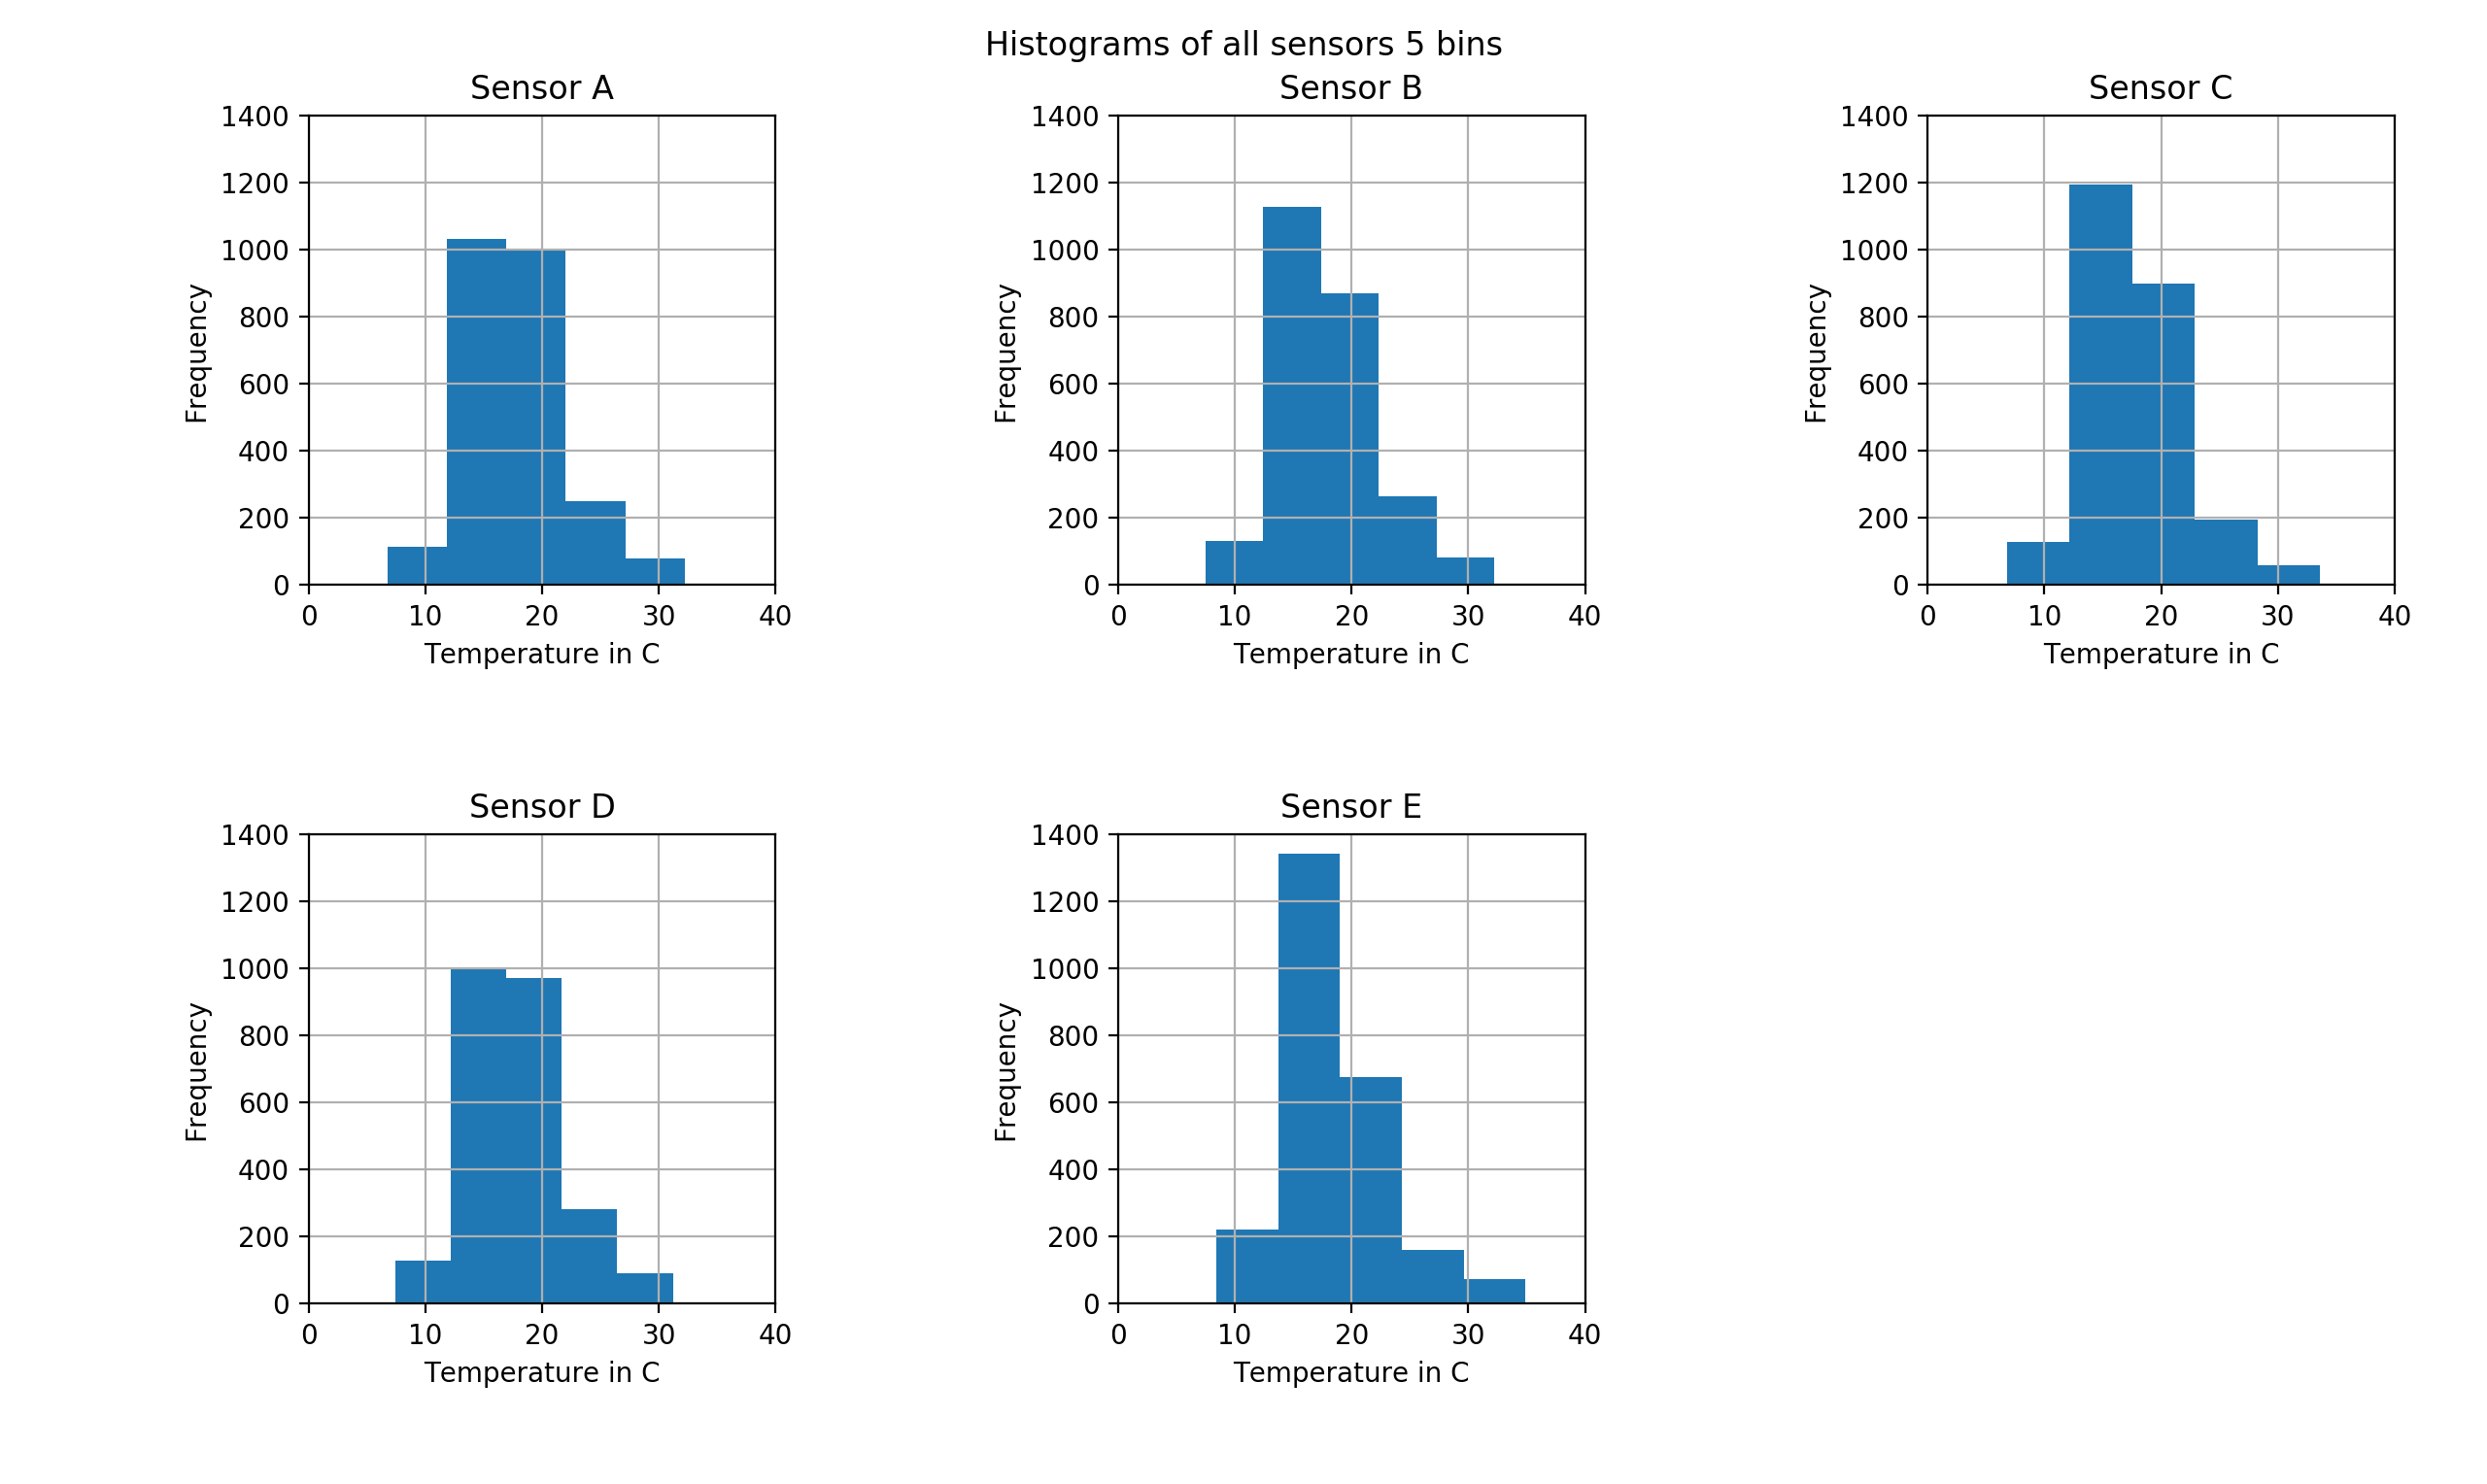
\includegraphics[width=\textwidth]{histogram_5_bins}

        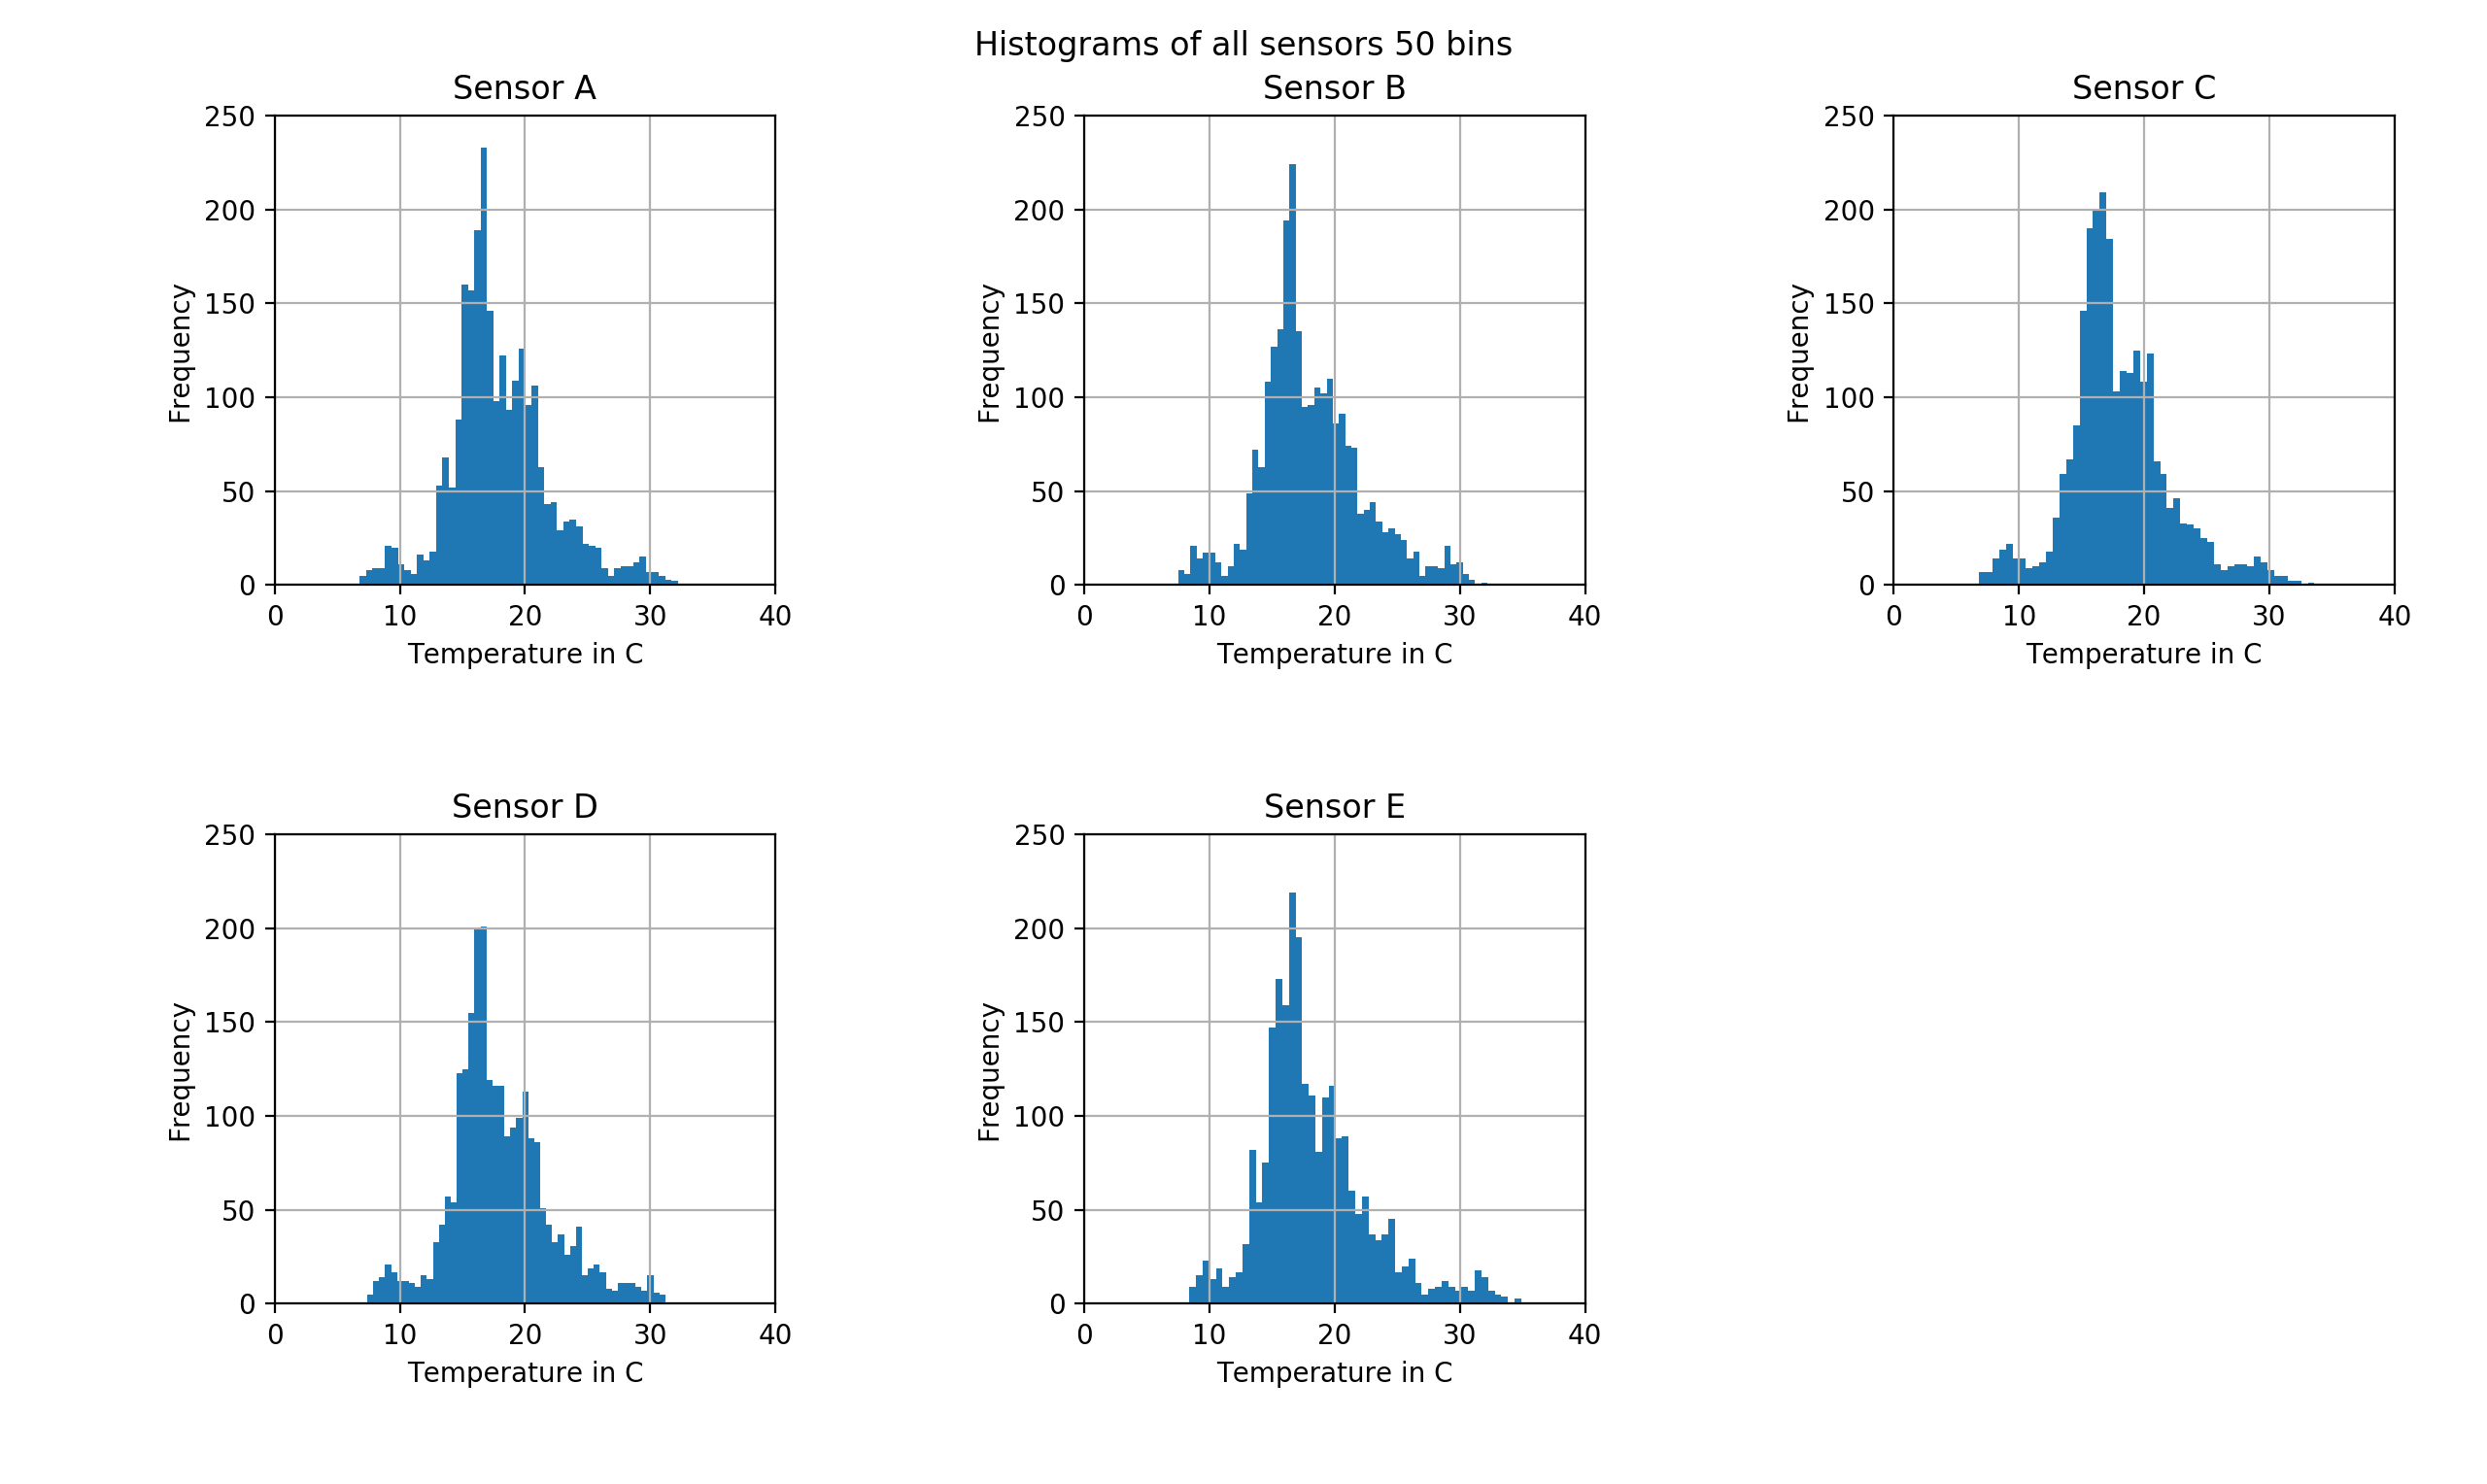
\includegraphics[width=\textwidth]{histogram_50_bins}


\section{A2}

Some other text here.

\section{A3}

\section{A4}



\end{document}